\documentclass[border=10pt]{standalone}
\usepackage[svgnames]{xcolor}
\usepackage{amsmath}
\usepackage{pgfplots}
\pgfplotsset{compat=newest}
\usepackage[sfdefault]{FiraSans}
\usepackage{FiraMono}
\renewcommand*\familydefault{\sfdefault}
\begin{document}
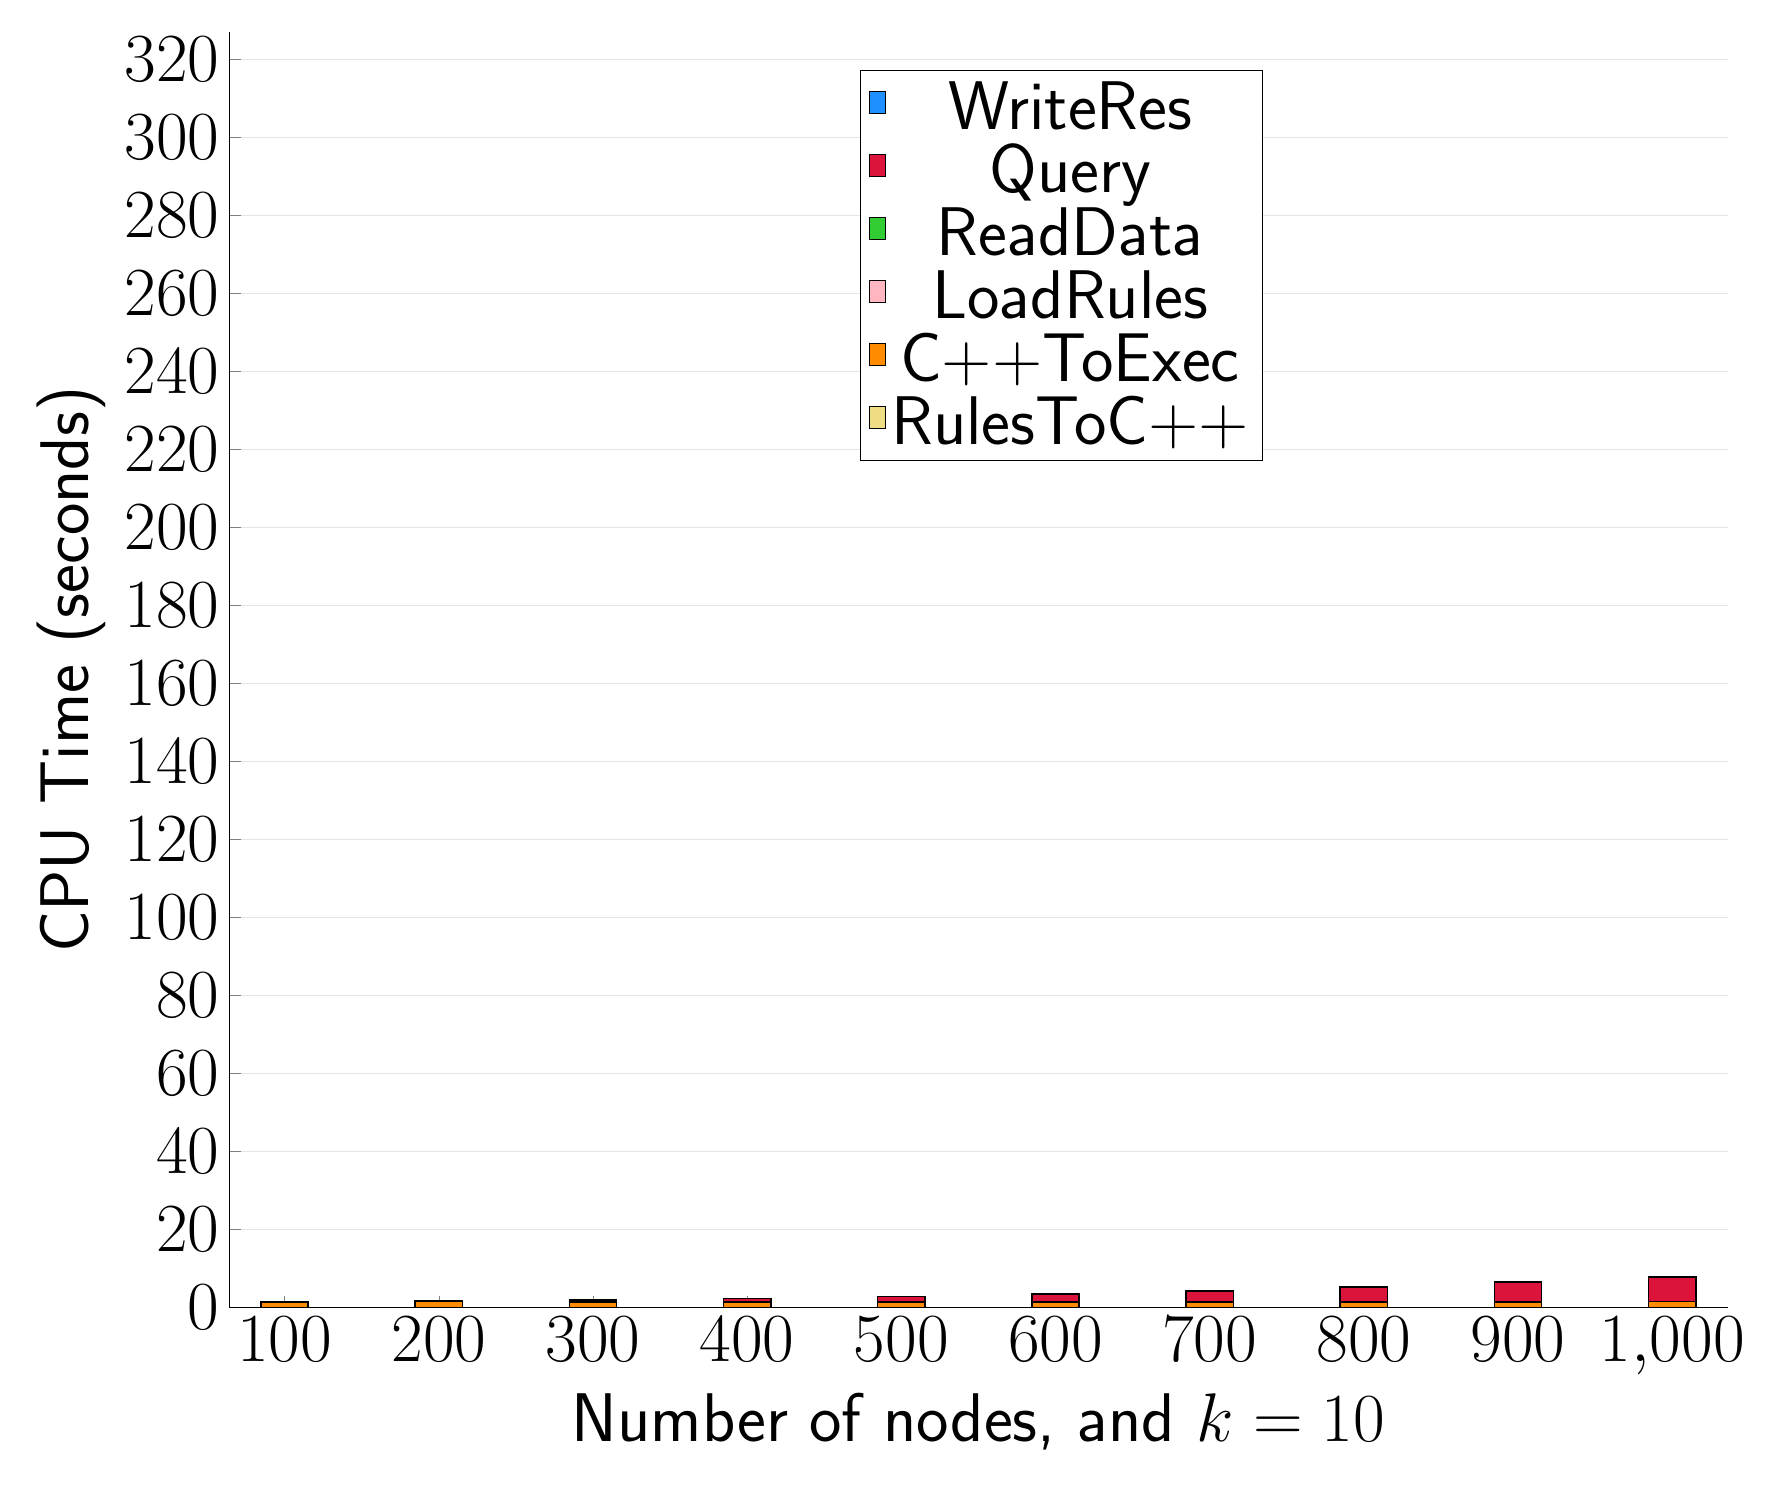
\begin{tikzpicture}
\begin{axis}[
   ybar stacked,
   width=1.7\textwidth,
   bar width=0.6cm,
   ymajorgrids, tick align=inside,
   major grid style={draw=gray!20},
   xtick=data,
   ymin=0, ymax=326.9108,
   axis x line*=bottom,
   axis y line*=left,
   enlarge x limits=0.04,
   legend style={
       at={(0.69, 0.97)},
       anchor=north east,
       legend columns=1,
       font=\Huge,
   },
   ylabel={CPU Time (seconds)},
   xlabel={Number of nodes, and $k=10$},
   label style={font=\Huge},
   tick label style={font=\Huge},
]
\addlegendimage{fill=DodgerBlue, draw=black, line width=0.2pt}
\addlegendentry{WriteRes}
\addlegendimage{fill=Crimson, draw=black, line width=0.2pt}
\addlegendentry{Query}
\addlegendimage{fill=LimeGreen, draw=black, line width=0.2pt}
\addlegendentry{ReadData}
\addlegendimage{fill=LightPink, draw=black, line width=0.2pt}
\addlegendentry{LoadRules}
\addlegendimage{fill=DarkOrange, draw=black, line width=0.2pt}
\addlegendentry{C++ToExec}
\addlegendimage{fill=LightGoldenrod, draw=black, line width=0.2pt}
\addlegendentry{RulesToC++}
\addplot +[fill=LightGoldenrod, draw=black, line width=0.55pt] coordinates {
(100, 0.010000000000000002)
(200, 0.004000000000000001)
(300, 0.006000000000000001)
(400, 0.004000000000000001)
(500, 0.006000000000000001)
(600, 0.0020000000000000005)
(700, 0.006000000000000001)
(800, 0.006000000000000001)
(900, 0.008000000000000002)
(1000, 0.0020000000000000005)
};
\addplot +[fill=DarkOrange, draw=black, line width=0.55pt] coordinates {
(100, 1.47)
(200, 1.496)
(300, 1.462)
(400, 1.464)
(500, 1.454)
(600, 1.4700000000000002)
(700, 1.468)
(800, 1.472)
(900, 1.472)
(1000, 1.484)
};
\addplot +[fill=LightPink, draw=black, line width=0.55pt] coordinates {
(100, 0.000165)
(200, 0.0001376)
(300, 0.00014439999999999999)
(400, 0.00012759999999999998)
(500, 0.0001564)
(600, 0.0001672)
(700, 0.0001808)
(800, 0.0001568)
(900, 0.0001678)
(1000, 0.00016340000000000001)
};
\addplot +[fill=LimeGreen, draw=black, line width=0.55pt] coordinates {
(100, 0.004372)
(200, 0.0058758000000000005)
(300, 0.0087692)
(400, 0.011111600000000001)
(500, 0.0149098)
(600, 0.0173258)
(700, 0.0222714)
(800, 0.023103)
(900, 0.0250172)
(1000, 0.0282346)
};
\addplot +[fill=Crimson, draw=black, line width=0.55pt] coordinates {
(100, 0.05403539999999999)
(200, 0.17692979999999997)
(300, 0.4281956)
(400, 0.8213594000000001)
(500, 1.34391)
(600, 1.9943259999999998)
(700, 2.8015160000000003)
(800, 3.75514)
(900, 4.926844)
(1000, 6.171436)
};
\addplot +[fill=DodgerBlue, draw=black, line width=0.55pt] coordinates {
(100, 0.0026714)
(200, 0.008795800000000001)
(300, 0.0194888)
(400, 0.0344686)
(500, 0.05390079999999999)
(600, 0.076373)
(700, 0.10387760000000001)
(800, 0.13608340000000002)
(900, 0.1712678)
(1000, 0.21250180000000002)
};
\end{axis}
\end{tikzpicture}

\end{document}
